\subsection{Display de 7 Segmentos}

O display de 7 segmentos é o elemento responsável pela representação visual dos valores numéricos do cronômetro. Ele é composto por sete LEDs organizados em formato específico, capazes de formar os dígitos de 0 a 9 através de combinações binárias.

Cada segmento recebe um indentificador convencionado entre [A,B,C,D,E,F,G] e que é ativado individualmente com base em sinais de entrada. Dessa forma, o display atua como a camada final de saída do sistema.

\begin{figure}[H]
    \centering
    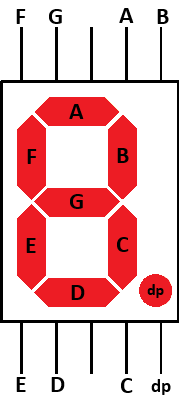
\includegraphics[width=0.3\linewidth]{images/7-segment-display.png}
    \caption{Display de 7 segmentos}
    \label{fig:7-segment-display}	
\end{figure}

Dessa forma, é possível construir um display de 7 segmentos no Minecraft utilizando lampadas e fios dispostos de forma similar a convenção padrão.

\begin{figure}[H]
    \centering
    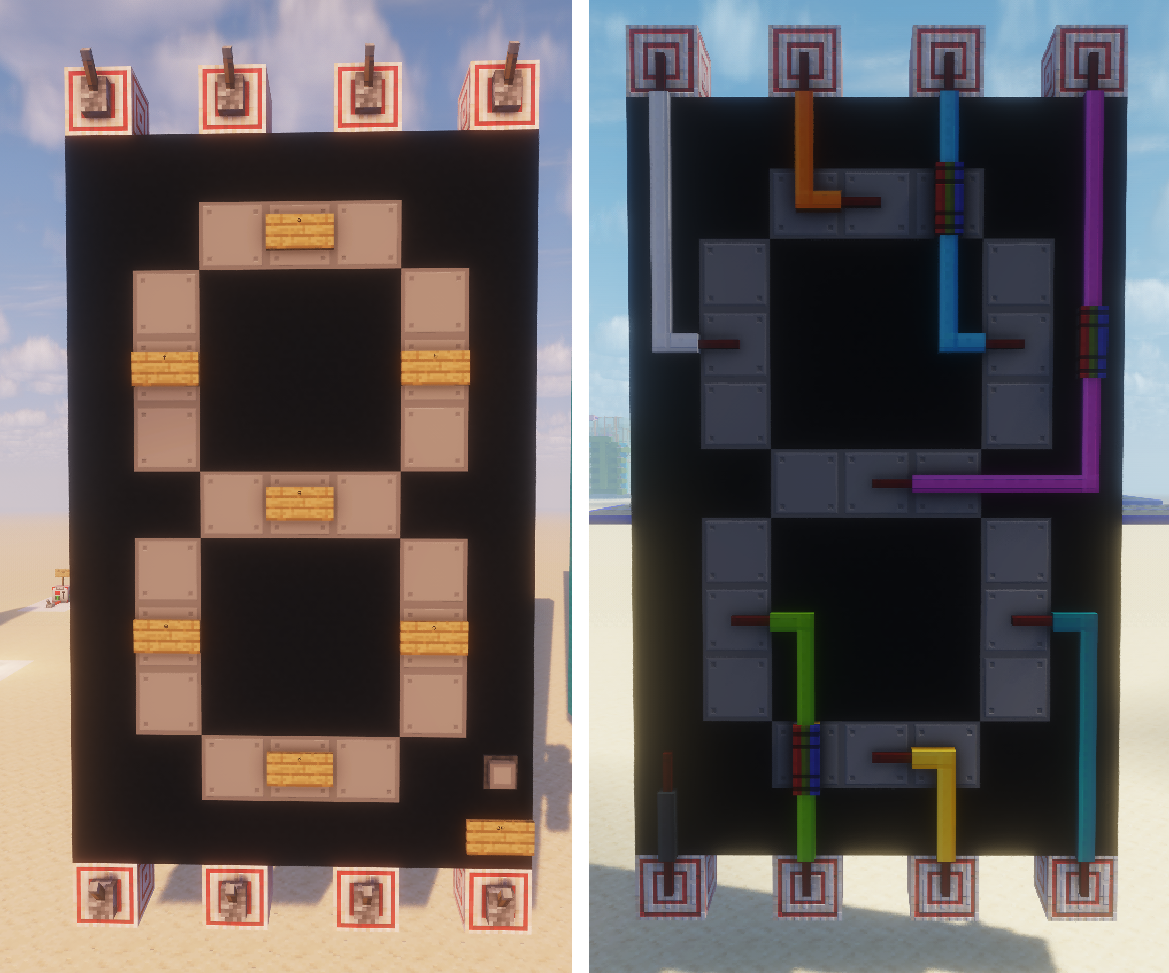
\includegraphics[width=0.6\linewidth]{images/7-segment-display-redstone.png}
    \caption{Display de 7 segmentos no Minecrat}
    \label{fig:7-segment-display-redstone}
\end{figure}